\documentclass[12pt,a4paper]{article}
\usepackage{graphicx}
\graphicspath{ {../Result/} }

\title{High Performance Computing Programming Exercise}
\author{Student:Shiyun Liu\\ s.liu18@imperial.ac.uk}
\date{ }

\begin{document}
\maketitle

\newpage

\section{Question 8}
\begin{figure}[h]
\centering
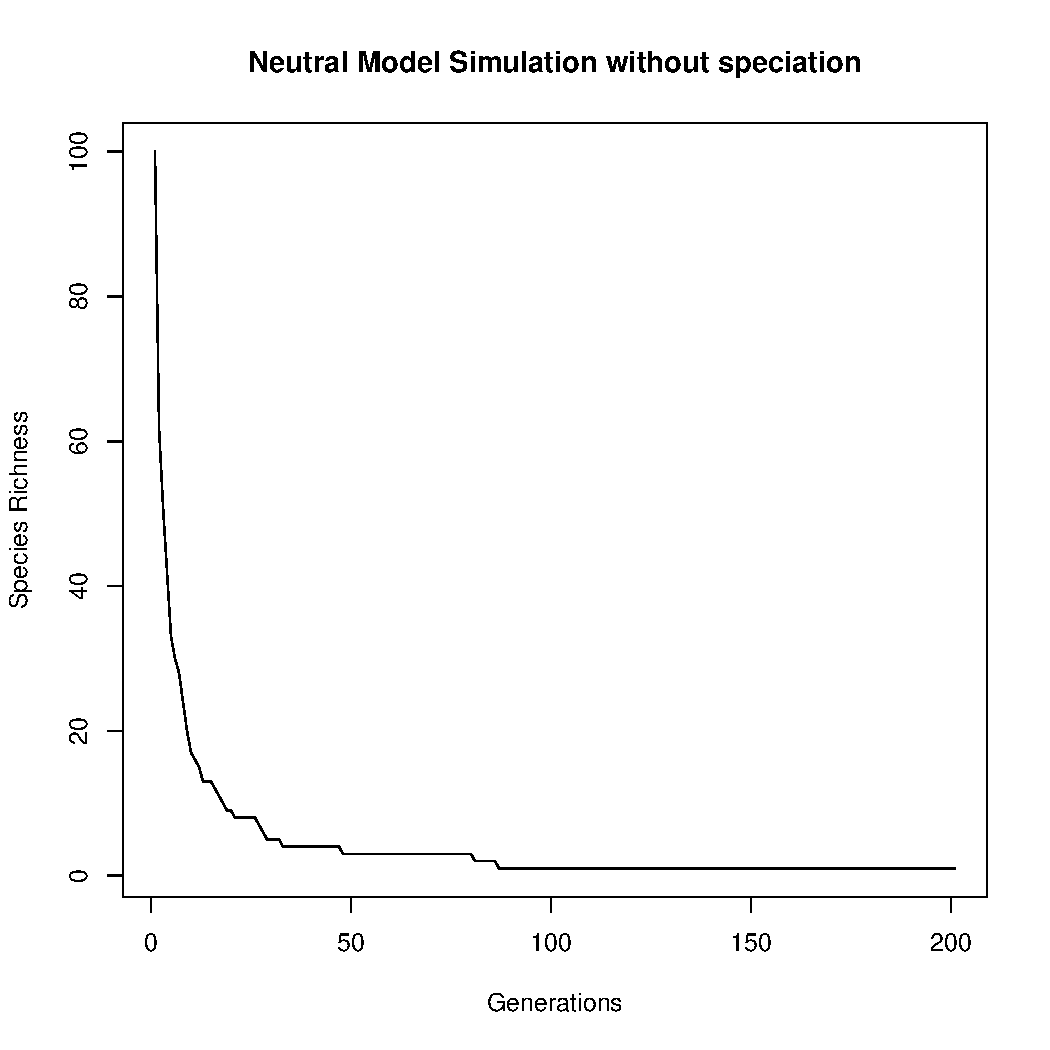
\includegraphics[width=\textwidth]{Q8Plot.pdf}
\end{figure}

Figure.Q8 This figure shows that species richness drops along with generation in a neutral model simulation without speciation beginning with maximal diversity. 
In this case, with community size of 100 and maximal initial diversity, the richness drops to minimal (1) in about 100 generations and then remains at that level.
\\
\\
The system will always converge to a equilibrium state of minimal species richness. 
Because in this simulation there is no speciation, therefore no new species introduced.
And the existing species will eventually be lost and replaced by other species in the system.
Therefore the species richness is expected to drop as generations go on and finally remain a single species system.

\newpage
\section{Question 12}
\begin{figure}[h]
\centering
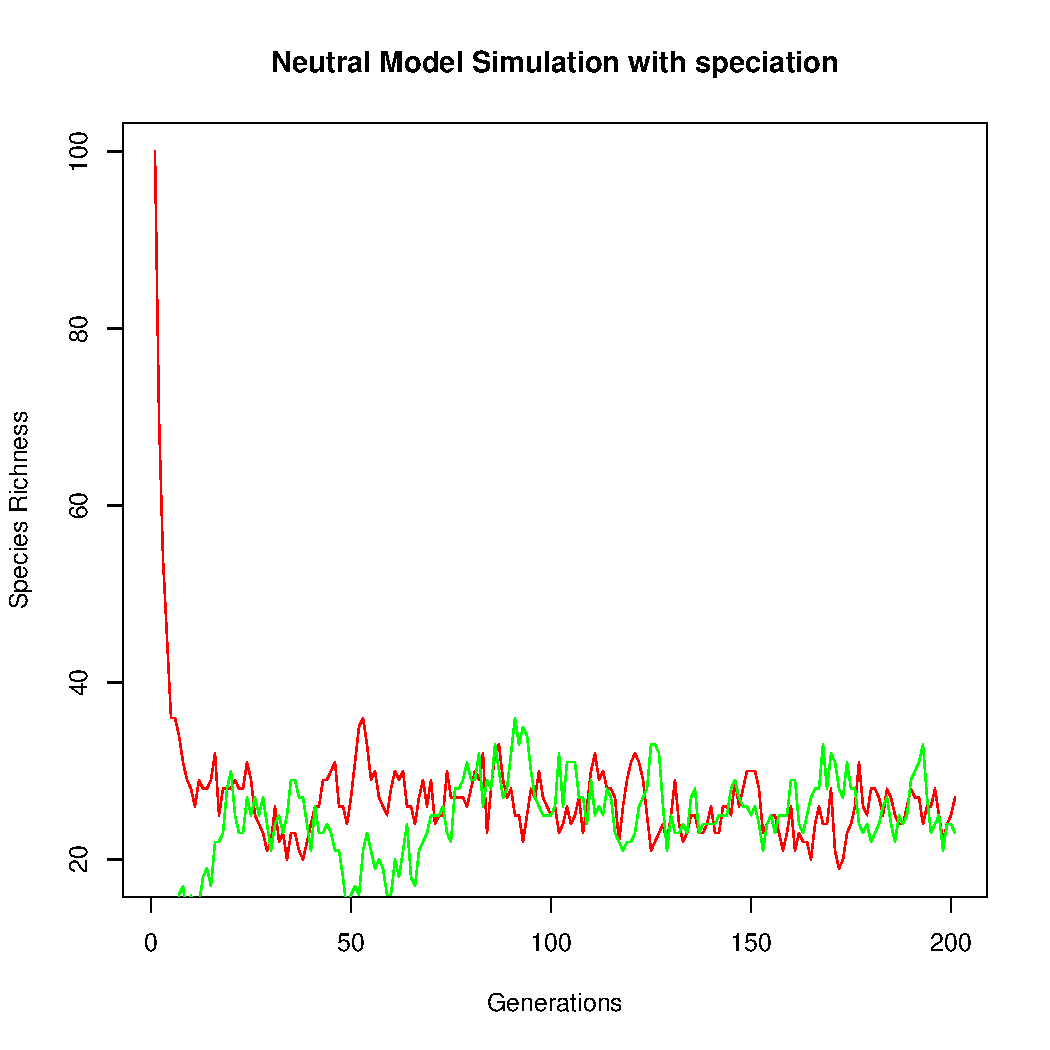
\includegraphics[width=\textwidth]{Q12Plot.pdf}
\end{figure}
Figure.Q12 This figure shows how species richness (for both 2 initial dicersity conditions) changes along with generation in a neutral model simulation with speciation.
Red line represents the initial condition of maximal diversity and the green line represents the minimal. Red line drops and green line increases during the burn-in period 
however they end up in similar fluctuating levels, around species richness of 25 in this case (community size 100, speciation rate 0.1 and burn-in generation about 30)
\\
\\
From this plot I found that the initial conditions do not affect the final state of neutral model simulation.
For both 2 communities with different initial species richness, they end up with similar fluctuating equilibrium in species richness.
\\
Because there is a certain speciation rate indicating the chance of introduction of new species in this system.
The final approximate species richness is influenced by the speciation rate and the initial community size regardless of the initial species richness.

\newpage

\section{Question 16}
\begin{figure}[h]
\centering
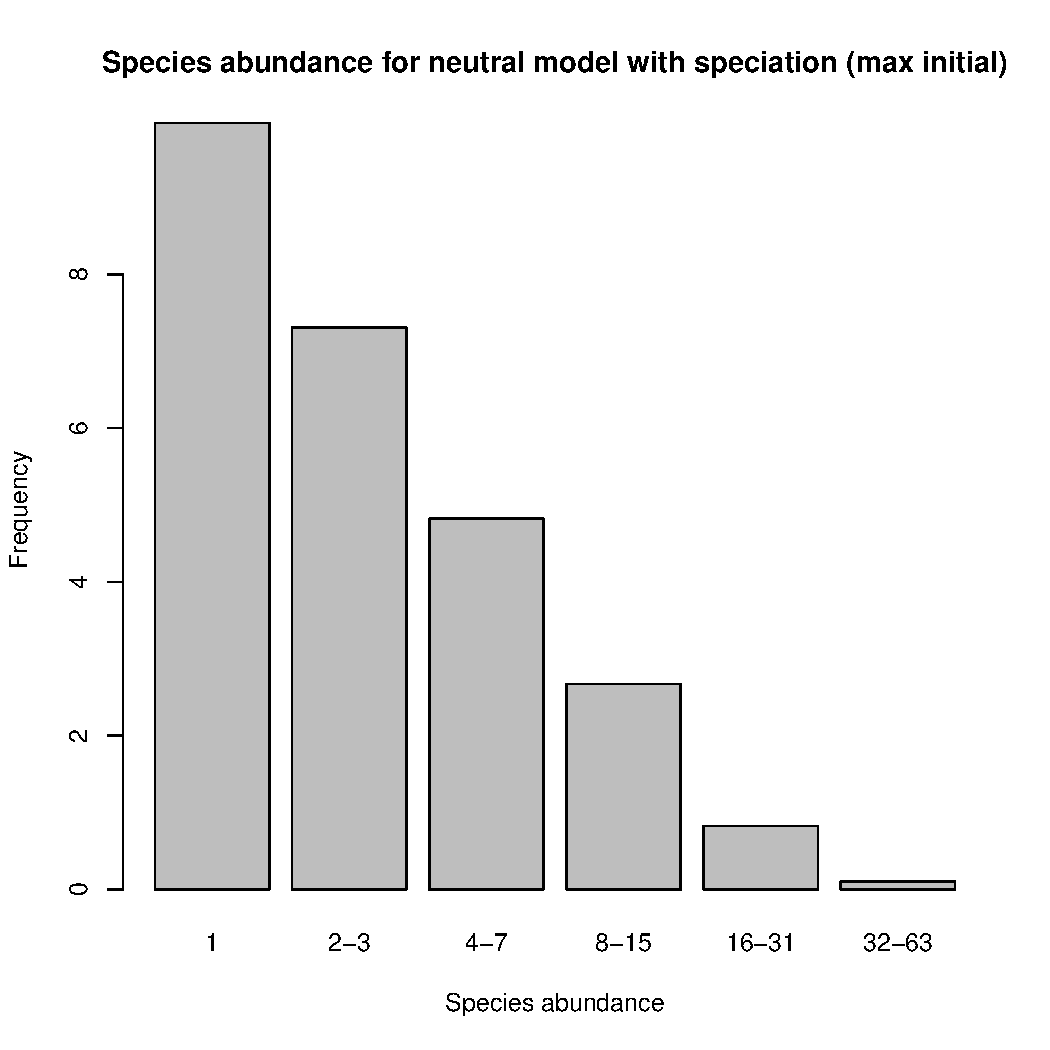
\includegraphics[width=\textwidth]{Q16Plot1.pdf}
\end{figure}
Figure.Q16a This graph shows the average species abundance (in octaves) for neutral model with speciation (max initial). 
It indicates that the majority of the species have small populations, only a few species have large populations.
\\
\\
\\
\\
\\
\\
\\
Figure.Q16b This graph shows the average species abundance (in octaves) for neutral model with speciation (max initial). 
It give same information as Figure.Q16a.
\begin{figure}[t]
\centering
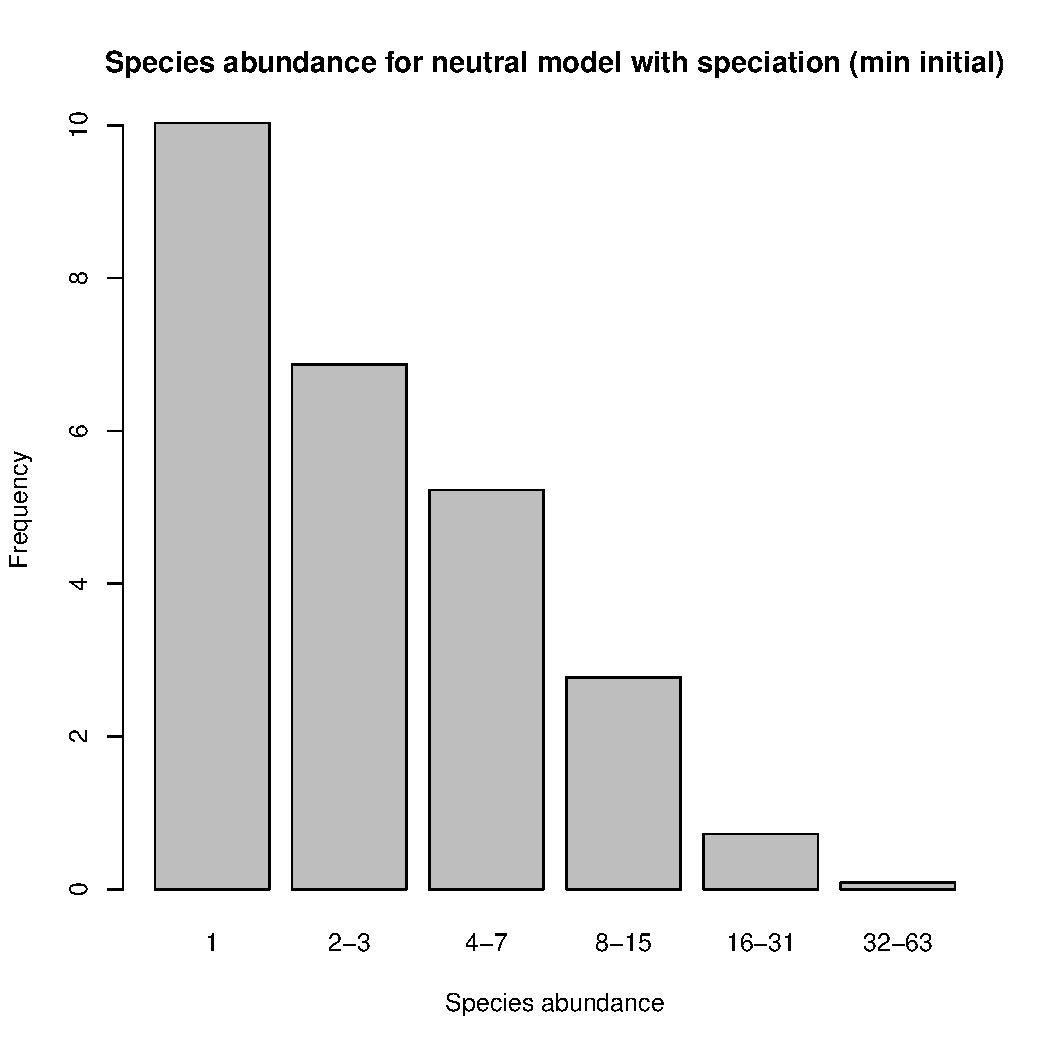
\includegraphics[width=\textwidth]{Q16Plot2.pdf}
\end{figure}
\\
\\
From these two plots we can tell that the initial condition does not influence the species abundance of the post burn-in period of simulated neutral theory simulation.
Because the speciation rate is pre-set and with generations last long enough, the abundance will only be influenced by the speciation rate and community size.


\newpage
\section{Challenge A}
\begin{figure}[h]
\centering
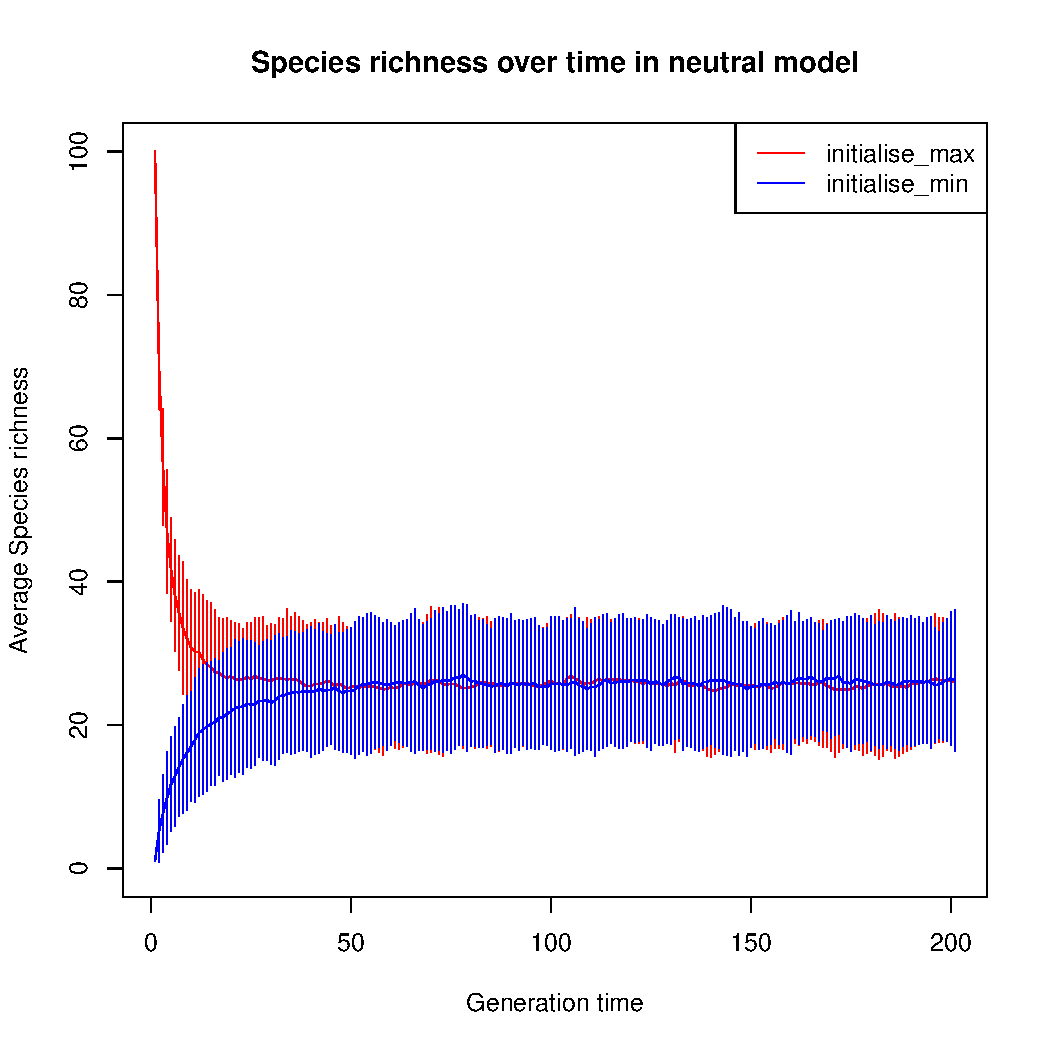
\includegraphics[width=\textwidth]{challengeA.pdf}
\end{figure}
Figure.ChallengeA This figure plots the species richness as a function of time in neutral model stimulation for both 2 initial
conditions. The confidence interval of 97.2% is added to the graph.
\\
\\
This graph indicates that the burn-in generation should be approximatly 50 (generations), 
which means for a community size of 100 and speciation rate 0.1, it takes about 50 generations to reach dynamic equilibrium, regardless of the initial species richness.
And the equilibrium level of species richness in this model stimulation is about 25 individuals per species.



\newpage
\section{Question 20}
\begin{figure}[h]
\centering
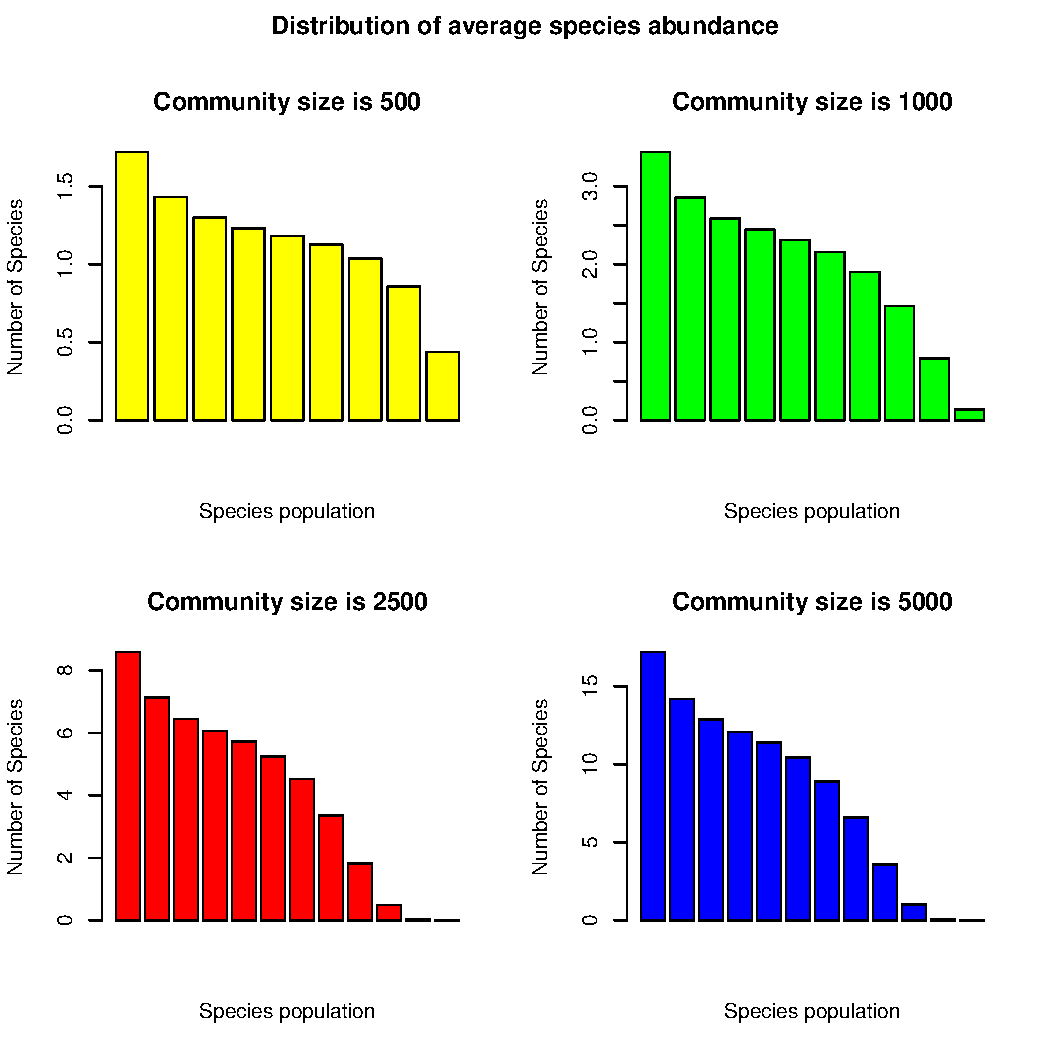
\includegraphics[width=\textwidth]{Q20Plot.pdf}
\end{figure}
Figure.Q20 This figure contains 4 barplots showing the species abundance (in octaves, post burn-in period) of 4 neutral model simulations (different community sizes) 
with speciation rate 0.003443. The data is generated by cluster run for 11.5 hours. (raw data is contained in the zip file and vectors used can be found in my R script).

\newpage
\section{Challenge C}
\begin{figure}[h]
\centering
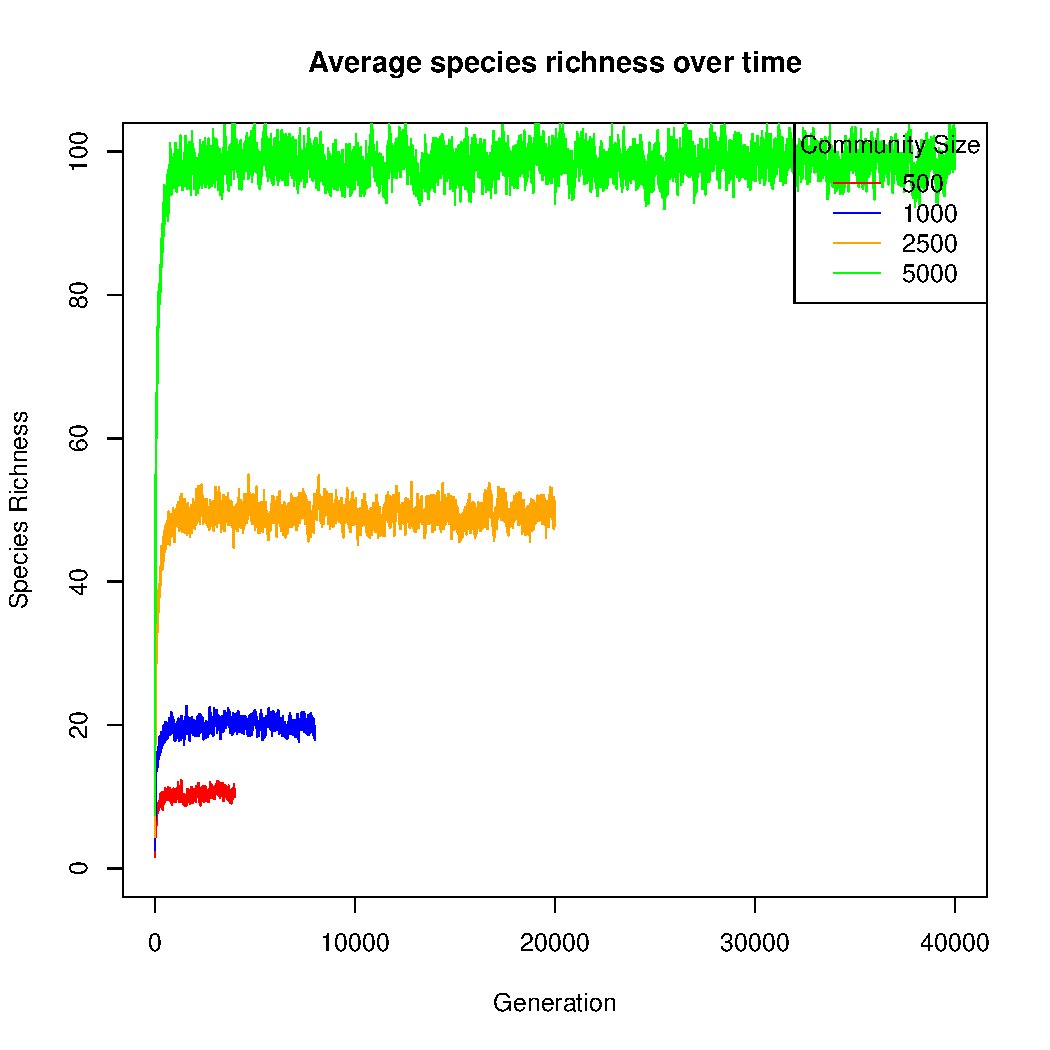
\includegraphics[width=\textwidth]{challengeC.pdf}
\end{figure}
Figure.ChallengeC This figure shows the mean species richness changes along with generation.



\newpage
\section{Question 21}
Fractal dimension D can be calculated by log(N)/log(r), whereas N is the dividing factor and r is the scaling factor.
\\
For the first object, N is 8 (area is 8 times bigger), r is 3 (length is 3 times larger), therefore D = log(8)/log(3) = 1.89
\\
For the second one, N is 20 (volume is 20 times bigger), r is 3 (length is 3 times larger), therefore D = log(20)/log(3) = 2.73
\newpage
\section{Question 22}
\begin{figure}[h]
\centering
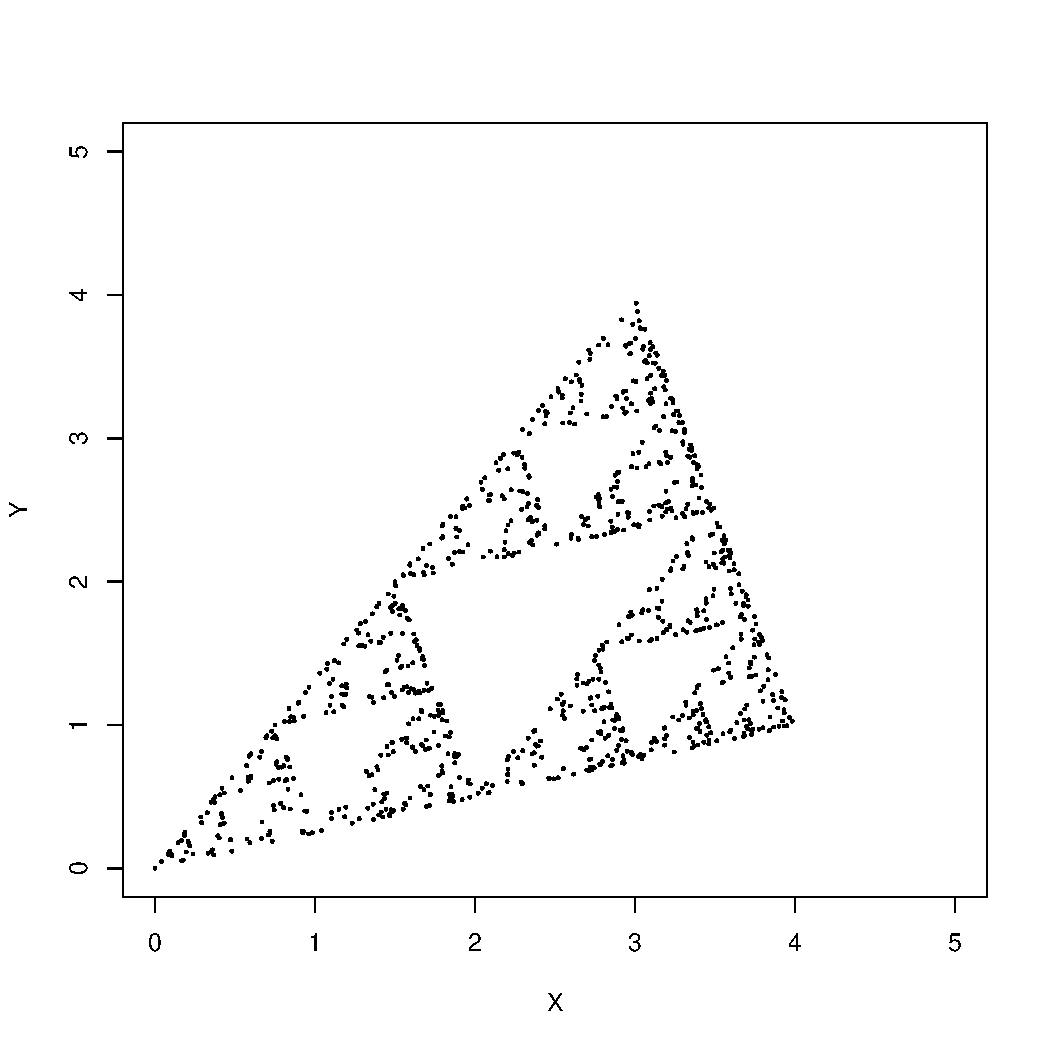
\includegraphics[width=\textwidth]{Q22Plot.pdf}
\end{figure}
Figure.Q22 This is the pattern generated by chaos game (100 times iteration)

\newpage
\section{Challenge E}
\begin{figure}[h]
\centering
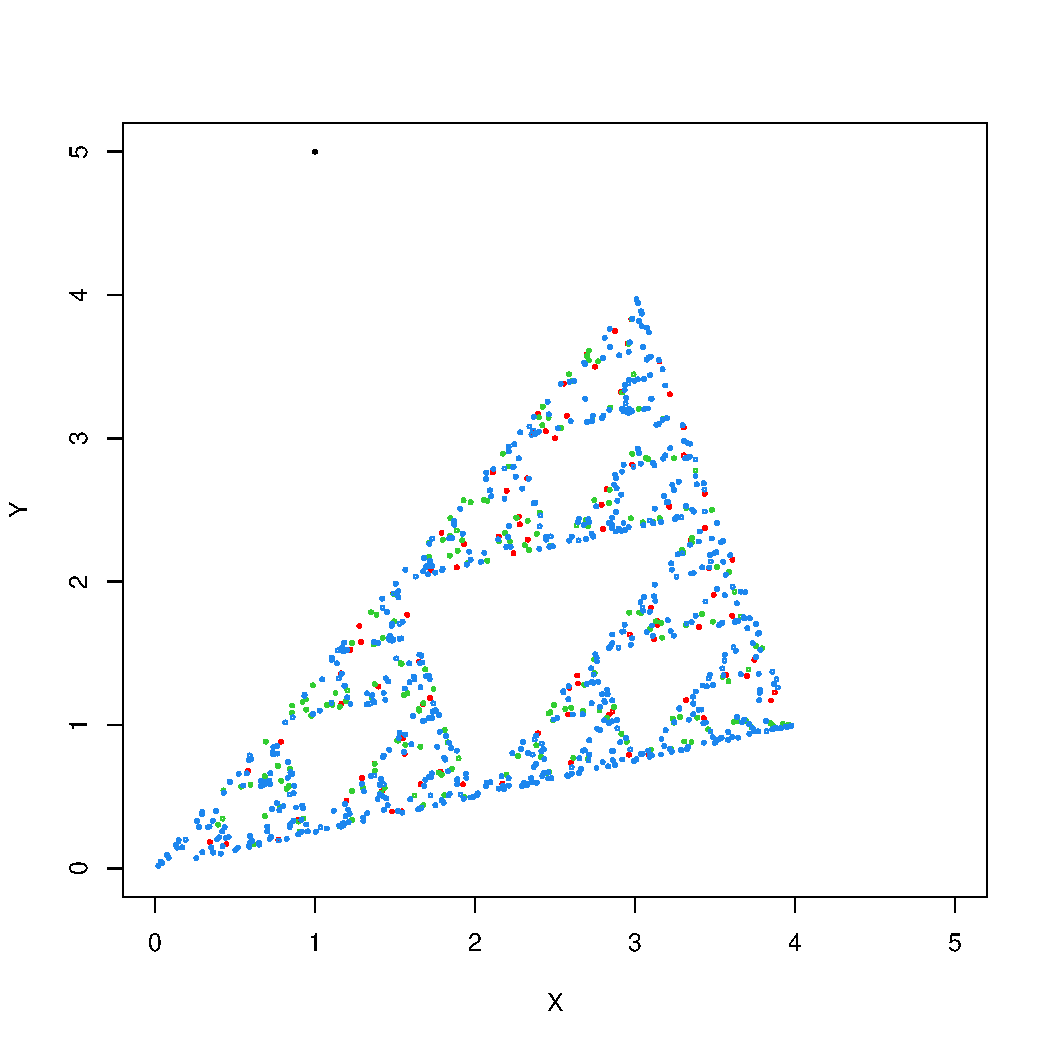
\includegraphics[width=\textwidth]{challengeE1.pdf}
\end{figure}
Figure.ChallengeE1 This chao game pattern was generated by a different initial position X and 
the first 100 points are colored red, the following 200 is colored green, the rest 700 is colored blue.
\\
\begin{figure}[h]
\centering
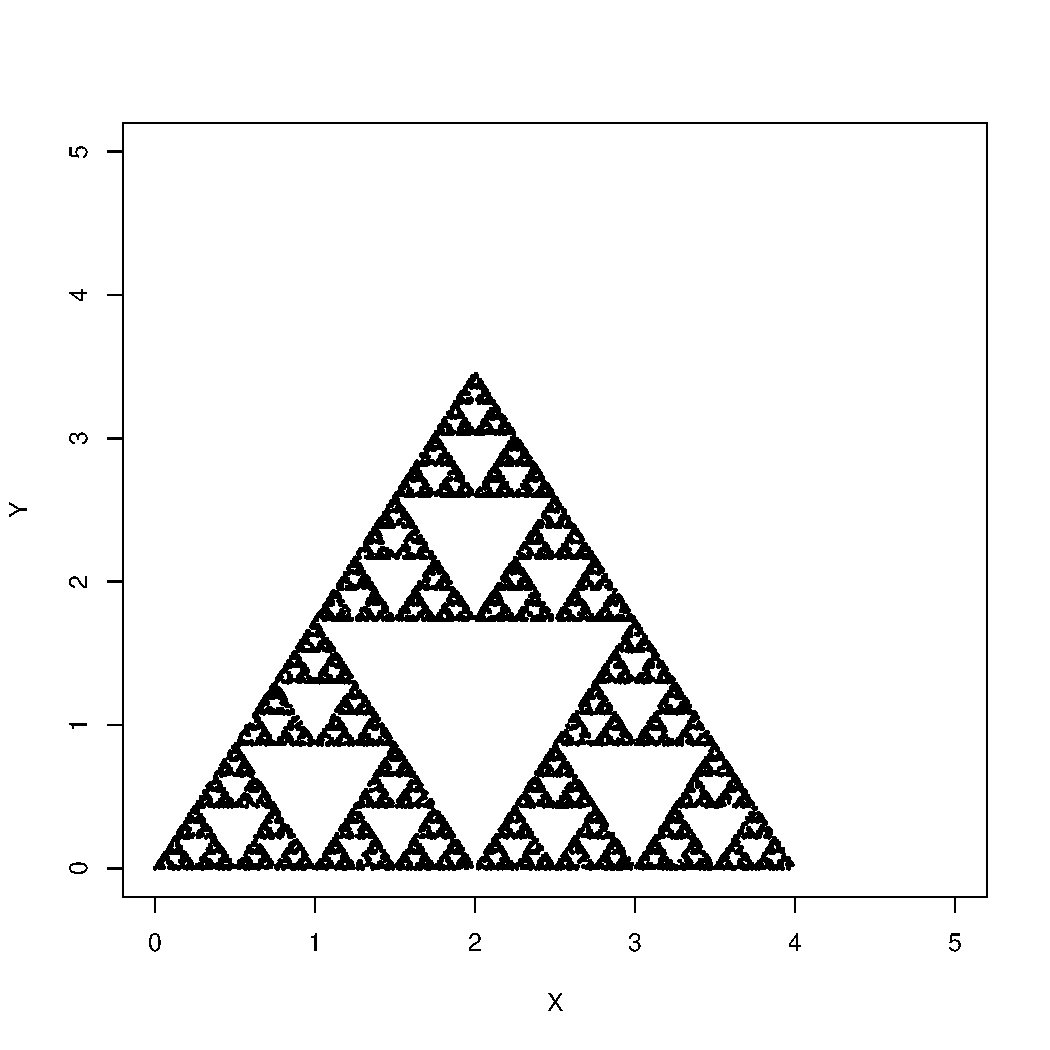
\includegraphics[width=\textwidth]{challengeE2.pdf}
\end{figure}
Figure.ChallengeE2 This classic Sierpinski Gasket pattern is generated based on chaos game but starting with the points
of an equilateral triangle as A,B,C.
\\
\\
From this chllenge E we can tell that the initial position X does not influence the pattern generated in this chaos game.
However the starting points A.B.C matters.


\section{Question 25}
Error message (evaluation nested too deeply: infinite recursion) occurs because this is an endless iteration.
The distance and direction can always get smaller and the computer have not idea when to stop, therefore runs into error.

\newpage
\section{Question 26}
\begin{figure}[h]
\centering
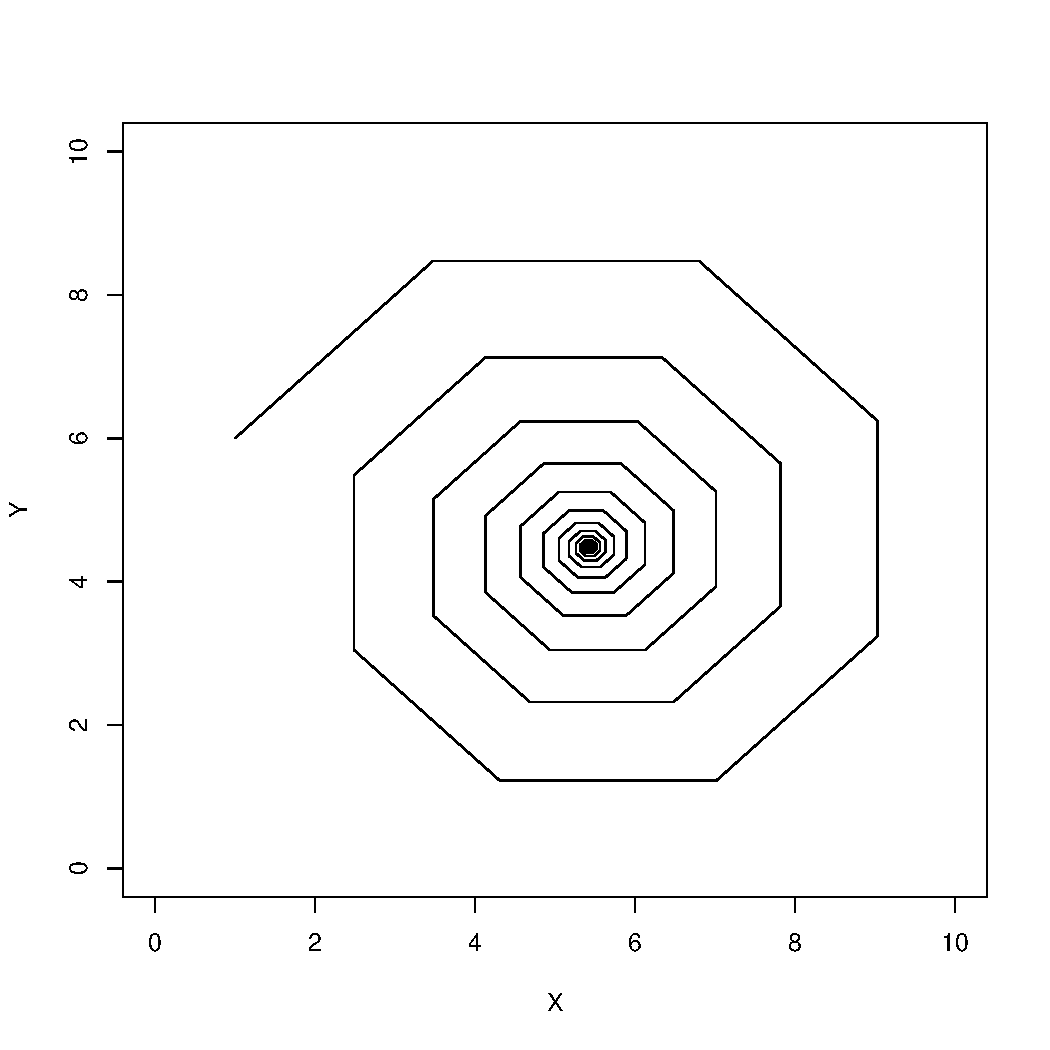
\includegraphics[width=\textwidth]{Q26Plot.pdf}
\end{figure}
Figure.Q26 This is a spiral pattern I generated with initial position (1,6), direction pi/4 (45 degree) and distance 3.5.

\newpage
\section{Question 27}
\begin{figure}[h]
\centering
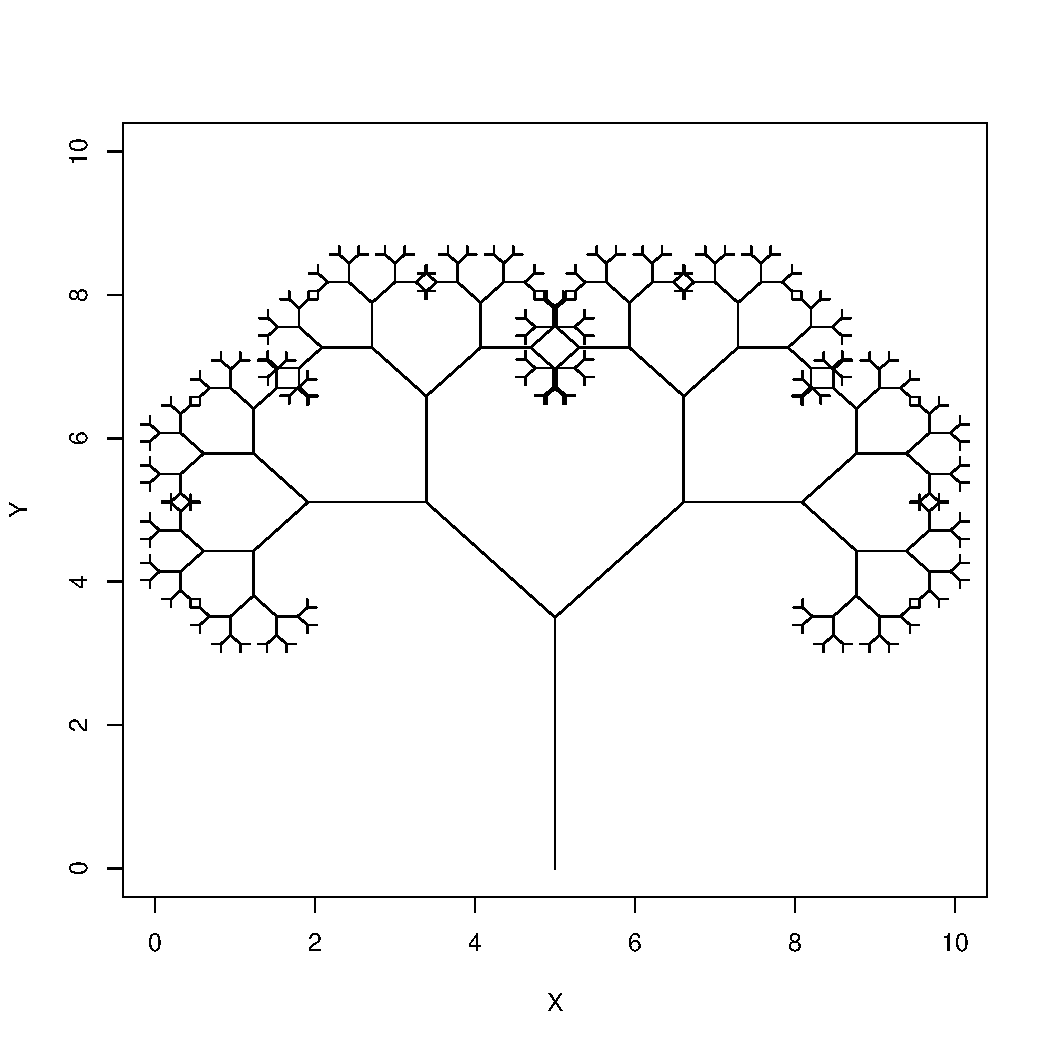
\includegraphics[width=\textwidth]{Q27Plot.pdf}
\end{figure}
Figure.Q27 This is a tree pattern I generated with initial position (5,0), direction pi/2 (90 degree) and distance 3.5.

\newpage
\section{Question 29}
\begin{figure}[h]
\centering
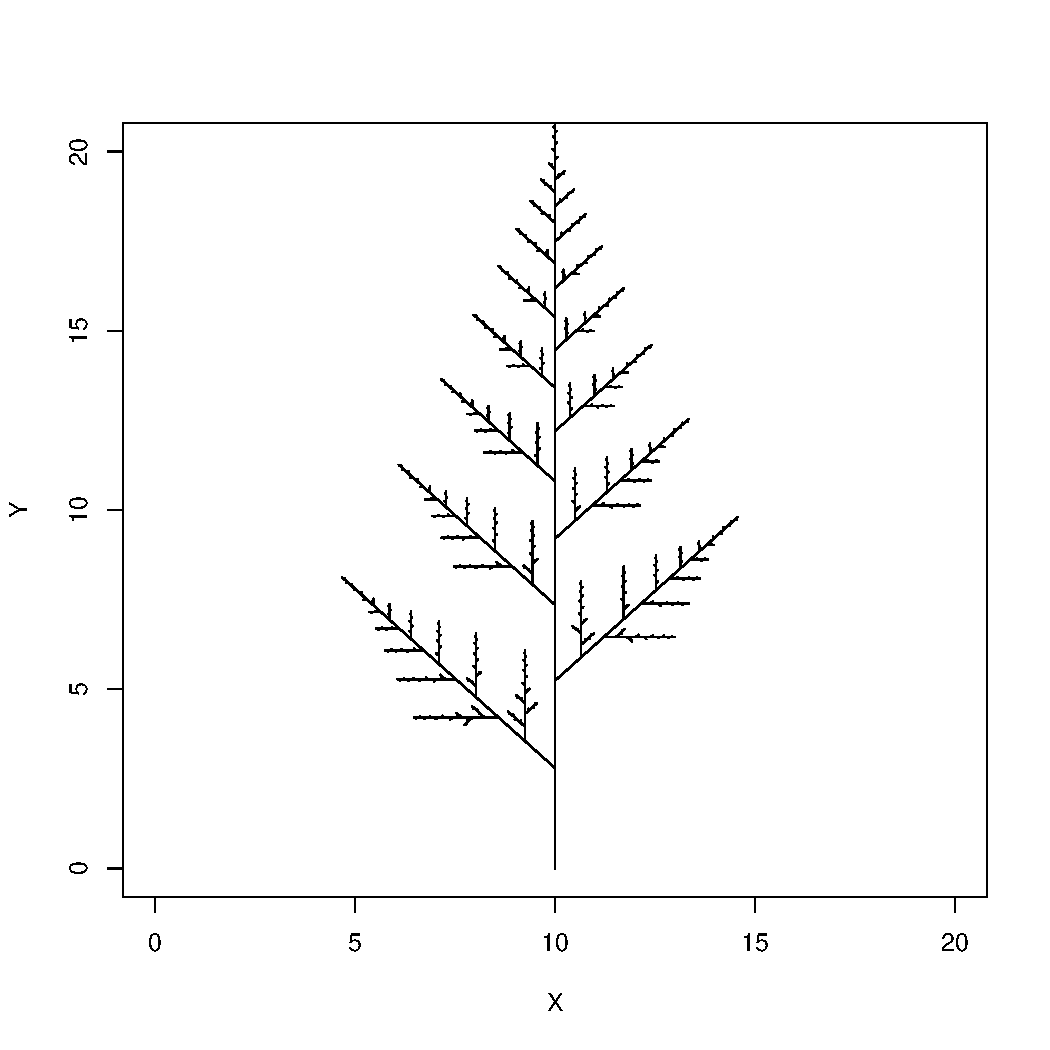
\includegraphics[width=\textwidth]{Q29Plot.pdf}
\end{figure}
Figure.Q29 This is a fern pattern I generated with initial position (10,0), direction pi/2 (90 degree) and distance 2.8.

\newpage
\section{Challenge F}
\begin{figure}[h]
\centering
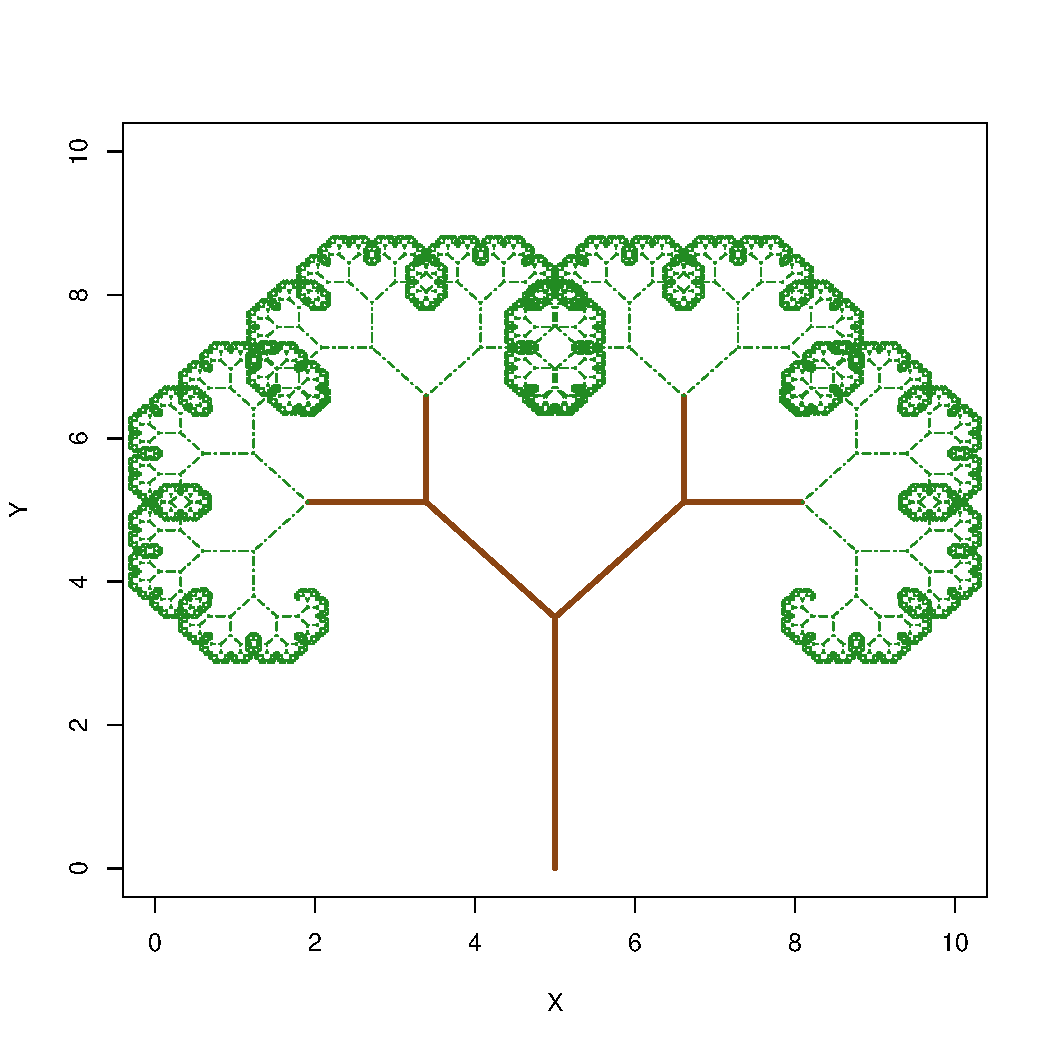
\includegraphics[width=\textwidth]{challengeF1.pdf}
\end{figure}
Figure.ChallengeF1 This is a prettier tree pattern generated with different colors and types of the lines allocated to different iterations.
\\
\\
\\
\\
\\
\\
\\
\\
\\
\begin{figure}[t]
\centering
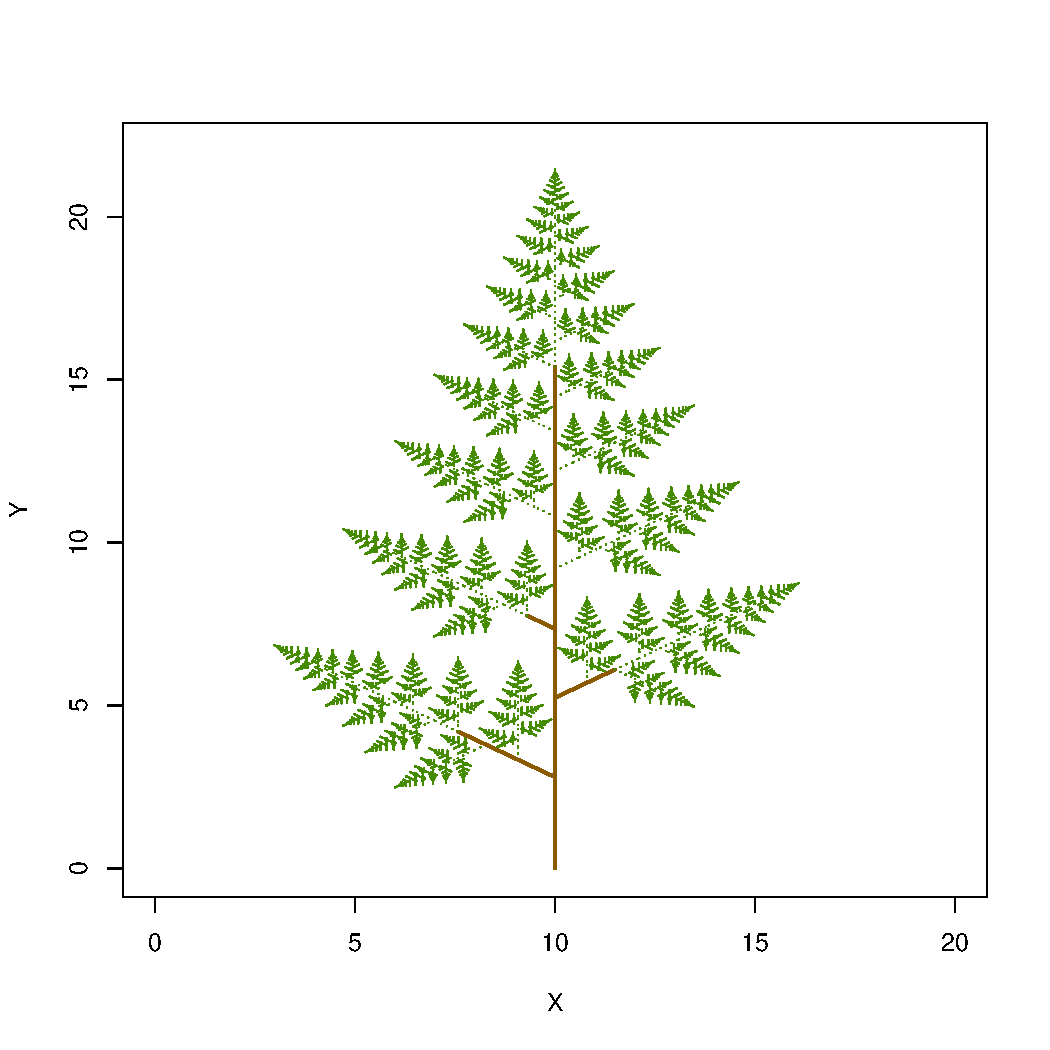
\includegraphics[width=\textwidth]{challengeF2.pdf}
\end{figure}
Figure.ChallengeF2 This is a prettier fern pattern generated with different colors and types of the lines allocated to different iterations, and also altered direction.
\\
As the value of e get smaller, the time required to produce the image becomes longer but a more detailed image produced.



\end{document}